\documentclass[11pt,a4paper]{article}

% -----------------------------------------------------------------------------
% Packages and document settings
% -----------------------------------------------------------------------------
\usepackage[T1]{fontenc}
\usepackage[utf8]{inputenc}
\usepackage[english]{babel}
\usepackage{lmodern}
\usepackage{microtype}
\usepackage[a4paper,margin=2.0cm]{geometry}
\usepackage{setspace}
\usepackage{graphicx}
\usepackage{booktabs}
\usepackage{array}
\usepackage{threeparttable}
\usepackage{caption}
\usepackage{subcaption}
\usepackage{float}
\usepackage{siunitx}
\usepackage{amsmath}
\usepackage{amssymb}
\usepackage{xcolor}
\usepackage{natbib}
\usepackage[hidelinks]{hyperref}
\usepackage{fancyhdr}

\graphicspath{
  {../../outputs/paper/figures/}
  {../../outputs/figures/}
  {outputs/paper/figures/}
  {outputs/figures/}
}

\sisetup{
  round-mode=places,
  round-precision=3,
  table-number-alignment=center
}

\captionsetup{
  font=small,
  labelfont=bf,
  justification=centering
}

\setstretch{1.03}
\setlength{\parindent}{0pt}
\setlength{\parskip}{0.35em}

\pagestyle{fancy}
\fancyhf{}
\fancyfoot[C]{\thepage}
\renewcommand{\headrulewidth}{0pt}

\hypersetup{
  pdftitle={Corporate Bankruptcy Risk Prediction with Machine Learning},
  pdfauthor={Berke Pehlivan},
  pdfsubject={Machine Learning for Finance research paper}
}

\newcommand{\repositoryurl}{https://github.com/Berke-Pehli/ml-finance-bankruptcy-analysis}

% -----------------------------------------------------------------------------
% Title information
% -----------------------------------------------------------------------------
\title{\textbf{Corporate Bankruptcy Risk Prediction\\with Machine Learning}\\[0.6em]
\large Comparing Interpretable Logistic Regression and Tree-Based Models}
\author{Berke Pehlivan\\
\small Matriculation No.: 50266988\\
\small Institutional email: \href{mailto:s36bpehl@uni-bonn.de}{s36bpehl@uni-bonn.de}\\
\small GitHub repository: \url{\repositoryurl}\\
\small Machine Learning for Finance\\
\small University of Bonn}
\date{Academic Year 2025/2026}

\begin{document}

\pagenumbering{gobble}

\begin{titlepage}
  \centering
  \vspace*{2.5cm}
  {\LARGE\bfseries Corporate Bankruptcy Risk Prediction\\[0.25em]
  with Machine Learning\par}
  \vspace{0.8cm}
  {\large Comparing Interpretable Logistic Regression\\
  and Tree-Based Models\par}
  \vfill
  {\large Berke Pehlivan\par}
  \vspace{0.3cm}
  {\normalsize Matriculation No.: 50266988\par}
  {\normalsize Institutional email: \href{mailto:s36bpehl@uni-bonn.de}{s36bpehl@uni-bonn.de}\par}
  {\normalsize GitHub repository: \url{\repositoryurl}\par}
  \vspace{0.3cm}
  {\normalsize Machine Learning for Finance\par}
  {\normalsize University of Bonn\par}
  {\normalsize Instructor: Ivan Gufler, Ph.D.\par}
  {\normalsize Academic Year 2025/2026\par}
  \vfill
\end{titlepage}

\pagenumbering{arabic}

% -----------------------------------------------------------------------------
% Main paper
% -----------------------------------------------------------------------------
\section{Introduction}
\label{sec:introduction}

\subsection{Financial motivation}

Corporate bankruptcy is an important problem for lenders, investors, auditors,
and risk managers. A firm's failure can impose losses on creditors and
shareholders. It can also disrupt relationships with employees, suppliers, and
other firms. Financial statements provide structured information about assets,
liabilities, revenues, expenses, and profitability. These variables may contain
signals of financial distress, so statistical learning can be used to study
bankruptcy risk. Early research showed
that accounting variables can help distinguish distressed from healthy firms
\citep{altman1968}. Later work studied bankruptcy risk in a probabilistic
classification framework \citep{ohlson1980}.

Despite this long research history, bankruptcy classification remains difficult.
The first difficulty is class imbalance. Failure is rare, so a model can achieve
high overall accuracy by predicting that almost every observation is alive. Such
a model may look successful even though it detects none of the failed
observations. A second difficulty is the structure of financial statement data.
Financial variables are often correlated, measured on different scales, and
partly affected by firm size. The relationship between accounting variables and
failure may also be nonlinear or depend on interactions. A third difficulty is
economic interpretation. Missing a failed firm can be costly, but flagging too
many healthy firms can make a screening system impractical.

For these reasons, evaluation is as important as model fitting. Accuracy is
reported, but it is not the main criterion in this imbalanced setting. The paper
therefore emphasizes failed-class precision, recall, F1-score, balanced
accuracy, ROC-AUC, and average precision, reported as PR-AUC. Precision--recall
analysis is especially useful when the negative class is much larger than the
positive class, because it shows the false-positive burden more directly
\citep{davis2006}. The classification threshold is also treated as a decision
choice rather than as an automatically optimal value.

\subsection{Research question and contribution}

This paper investigates the following research question:

\begin{quote}
\emph{How effectively can interpretable and tree-based machine-learning models
distinguish failed from alive company-year observations for previously unseen
companies, and what trade-offs arise between failure detection and false
alarms?}
\end{quote}

The analysis uses the American corporate bankruptcy dataset introduced by
\citet{lombardo2022}. The working sample contains 78,682 company-year
observations from 8,971 anonymized companies between 1999 and 2018, with 18
financial predictors and a binary failed/alive target. Because companies may
appear in multiple years, observations are split at the company level. This
prevents the same company from appearing in both training and final-test data
and reduces the risk that persistent company characteristics create an
artificially favorable evaluation. The design tests generalization to unseen
companies; it is not presented as a chronological forecasting backtest.

The empirical comparison begins with a majority-class baseline, which
demonstrates why accuracy alone is misleading. Logistic Regression provides the
main interpretable benchmark. L1- and L2-regularized variants test whether
coefficient shrinkage helps when predictors are correlated. A Decision Tree,
Random Forest, and Gradient Boosting model then test whether nonlinear rules and
interactions improve performance. Together, these models allow a comparison
between a simple interpretable model and more flexible tree-based methods. This
makes it possible to compare models that differ in flexibility and
interpretability \citep{james2023}. A PCA plus Logistic Regression
specification is included as a dimension-reduction extension, not as the main
model.

The paper focuses on three main points. First, it compares interpretable and
tree-based models in a reproducible way and avoids company overlap between the
training and test data. Second, it uses metrics that focus on the failed class
and keeps the final test set separate for the main comparison. Third, it
connects the model results to financial screening by discussing classification
errors, threshold trade-offs, coefficients, and feature importance. The linked
GitHub repository contains the notebooks, data, and saved outputs needed to
reproduce the tables and figures. The results are interpreted as predictive
associations rather than causal effects. The project is intended as an
educational model comparison and not as a system for automatic credit or
investment decisions.

\section{Data}
\label{sec:data}

\subsection{Dataset and unit of observation}

The project uses the American corporate bankruptcy dataset published by
\citet{lombardo2022}. It contains accounting information for public companies
listed in the United States. The version used here has 78,682 company-year
observations covering the years 1999 to 2018. It contains 8,971 anonymized
company identifiers, 18 financial predictors, a year variable, and a company
status. The data summary reports no missing values and no duplicated rows.

One row represents one company in one year. The same company can therefore
appear in several years. This matters for the train-test design. A random
row-level split could place observations from the same company in both training
and test data. The model could then benefit from company-specific information
already seen during training. To reduce this risk, the project assigns whole
companies to the training or final-test sample. Section~\ref{sec:methodology}
explains the split in more detail.

The source data cover a long period in which both the set of listed companies
and the wider economic environment changed. The project does not use a
time-based holdout. The final test set contains unseen companies, but its
calendar years overlap with the training years. The results therefore show how
well the models work for unseen companies under this split, not how well they
would predict a later period.

\subsection{Target and financial predictors}

The original status is recorded as \texttt{alive} or \texttt{failed}. For
modeling, failed observations are coded as 1 and alive observations as 0. The
failed class is treated as the positive class throughout the analysis. The
company identifier and year are kept for splitting and reporting, but they are
not used as predictors. This leaves 18 financial inputs, labelled \texttt{X1}
to \texttt{X18} in the source file.

The predictors cover several parts of a company's financial position and
performance. They include current assets, inventory, receivables, market value,
and total assets; profitability measures such as EBITDA, EBIT, net income,
gross profit, and retained earnings; long-term debt, current liabilities, and
total liabilities; and activity measures such as sales, revenue, cost of goods
sold, and operating expenses. Depreciation and amortization is also included.
The models therefore use the reported financial values rather than newly created
financial ratios. The tables and figures use readable names so that the outputs
can be discussed in financial terms.

The variables have very different scales. Several also describe related parts of
the same financial statements. For example, revenue and net sales are closely
connected, as are assets and liabilities. This matters for Logistic Regression
because coefficient size depends on measurement scale. Correlated predictors can
also make individual coefficients less stable. The Logistic Regression and PCA
pipelines therefore standardize the predictors using parameters learned from the
training data. Tree-based models do not require this scaling.

\subsection{Class imbalance and descriptive evidence}

The target is strongly imbalanced. Of the 78,682 company-year observations,
73,462 are alive and 5,220 are failed. The failed class therefore represents
only 6.63\% of the full sample. Figure~\ref{fig:class-distribution} shows this
difference. A classifier that predicts every observation as alive would be
correct in more than 93\% of the full sample. However, it would detect no
failures. This is the main reason why the later evaluation does not rely on
accuracy alone.

\begin{figure}[H]
  \centering
  
\includegraphics[width=0.72\textwidth]{class_balance.png}
  \caption{Class distribution in the full dataset. The failed class accounts
  for 6.6\% of company-year observations.}
  \label{fig:class-distribution}
\end{figure}

The share of failed observations also changes over time. As shown in
Figure~\ref{fig:annual-failure-rate}, the observed rate rises from 7.16\% in
1999 to a peak of 9.40\% in 2003 and then generally declines, reaching 1.32\%
in 2018. This pattern should be interpreted carefully. It may reflect economic
conditions, changes in the companies included in the dataset, or the way status
is represented. The figure only describes the available sample. It does not show
that time caused the change in failure rates.

\begin{figure}[H]
  \centering
  
\includegraphics[width=0.82\textwidth]{annual_failure_rate.png}
  \caption{Observed annual failure rate in the full dataset, 1999--2018.}
  \label{fig:annual-failure-rate}
\end{figure}

Table~\ref{tab:financial-medians} compares the medians of six selected
financial variables. Medians are used because financial statement values are
often skewed and can contain very large observations. Failed observations have
lower median market value, net income, current assets, and retained earnings.
They have higher median long-term debt and total liabilities. These differences
make sense from a financial perspective, but they do not show that the variables
cause failure. They are simple comparisons between the two groups and do not
control for the other predictors.

\begin{table}[H]
  \centering
  \caption{Selected financial-variable medians by company status}
  \label{tab:financial-medians}
  \begin{threeparttable}
    \begin{tabular}{lrr}
      \toprule
      Financial variable & Alive median & Failed median \\
      \midrule
      Market value         & 240.90 & 117.80 \\
      Net income           &   2.07 &  -3.33 \\
      Total long-term debt &   7.09 &  18.44 \\
      Current assets       & 102.92 &  75.87 \\
      Total liabilities    &  80.74 &  97.04 \\
      Retained earnings    &  -0.17 & -25.51 \\
      \bottomrule
    \end{tabular}
    \begin{tablenotes}[flushleft]
      \footnotesize
      \item Notes: Values are shown in the units reported by the source
      dataset. The table is descriptive and does not imply causal effects.
    \end{tablenotes}
  \end{threeparttable}
\end{table}

\section{Methodology}
\label{sec:methodology}

\subsection{Company-level training, validation, and test design}

The full sample is first divided into training and final-test data with a
grouped random split. The company identifier is used as the group, so every row
from a company is assigned to the same side of the split. The split places 80\%
of companies in training and 20\% in the final test set. A fixed random seed of
42 is used so that the result can be reproduced. The training set contains
62,988 rows from 7,176 companies, while the final test set contains 15,694 rows
from 1,795 companies. The failure rates are 6.42\% and 7.50\%, respectively.

A second company-level split is then created inside the training set. This
inner split reserves 20\% of the training companies for validation. It produces
a model-fitting sample of 50,323 rows from 5,740 companies and a validation
sample of 12,665 rows from 1,436 companies. Hyperparameters are compared on the
validation sample using PR-AUC. The same validation predictions are later used
for the threshold analysis. The final test set is not used for model selection
or validation threshold analysis.

The final evaluation uses the fitted models from the inner model-fitting sample.
The validation rows are not added back for a final refit. This keeps the final
test comparison tied to the same fitted models that were chosen during
validation. The cost is that the final models use fewer observations than they
could have used. Refitting the selected specification on all non-test training
rows would be more data-efficient, but that alternative was not used here. This
point is considered again in the limitations section.

All random model components use the same seed. The implementation uses
scikit-learn pipelines and estimators \citep{pedregosa2011}. Pipelines are
important for Logistic Regression and PCA because standardization is learned
only from the fitting data and then applied to validation or test observations.
This prevents information from the validation or test data from entering the
preprocessing step.

\subsection{Majority-class baseline}

The first model is a majority-class baseline. It always predicts the most common
training label, which is \texttt{alive}. The baseline does not try to learn a
relationship between the financial variables and the target. Its purpose is to
give a simple reference point. Because alive observations are very common, this
rule achieves high accuracy while its recall for failures is zero. A useful
bankruptcy classifier should therefore be evaluated with more than overall
accuracy.

\subsection{Logistic Regression and regularization}

Logistic Regression is the main interpretable model. For observation $i$, the
model links the probability of failure $p_i$ to the financial predictors through

\begin{equation}
  \log\left(\frac{p_i}{1-p_i}\right)
  = \beta_0 + \beta_1 x_{i1} + \cdots + \beta_{18} x_{i18}.
\end{equation}

The left-hand side is the log-odds of failure. A positive coefficient is linked
to higher predicted failure log-odds when the other variables are held fixed. A
negative coefficient is linked to lower predicted failure log-odds. The
coefficients are not direct percentage-point changes in probability, and they
are not interpreted as causal effects.

Each Logistic Regression specification is placed after a standardization step.
The predictors therefore have mean zero and standard deviation one in the
model-fitting sample. This makes the regularization penalty comparable across
variables with different units. Balanced class weights give more importance to
errors on the minority failed class during fitting. They do not create
additional failed observations, rebalance the test set, directly choose the
classification threshold, or make the resulting scores calibrated real-world
bankruptcy probabilities.

Three Logistic Regression specifications are compared. The main benchmark uses
an L2 penalty with fixed $C=1$. L1 and L2 variants are added to check whether
regularization helps when predictors are correlated. The parameter $C$ is the
inverse of the regularization strength, so a smaller value means stronger
shrinkage. Separate L1 and L2 models compare
$C \in \{0.01, 0.1, 1, 10\}$ using validation PR-AUC. Both regularized models
select $C=0.1$. L1 regularization can set some coefficients exactly to zero. L2
regularization usually keeps all variables but shrinks their coefficients. These
methods can help when predictors are strongly related, although they can also
add some bias \citep{james2023}.

\subsection{Tree-based models}

Tree-based models are included because they can represent nonlinear patterns and
interactions without manually specifying them. The Decision Tree is the simplest
tree model in the comparison. It separates the observations by applying a
sequence of decision rules. Its depth and minimum leaf size control complexity. A deep tree
may fit the training data closely but can have high variance. The selected tree
has a maximum depth of 5 and at least 50 observations in each leaf. Balanced
class weights are used during fitting.

Random Forest is included to reduce the variance of a single tree. It averages
many trees fitted on resampled data. It also considers a random subset of
predictors at each split, which makes the trees less similar to each other
\citep{breiman2001}. The selected model uses 300 trees, no fixed maximum depth,
at least 50 observations per leaf, and the square root of the available
predictors at each split. Class weights are balanced separately within each
bootstrap sample.

Gradient Boosting is included as a second ensemble approach. It also combines
many trees, but it builds them in sequence. Each new tree is added to improve
the errors left by the existing ensemble \citep{friedman2001}. The learning
rate controls how much each new tree changes the model. The selected
specification uses 150 trees, a learning rate of 0.05, a maximum tree depth of
3, and at least 100 observations per leaf. The scikit-learn Gradient Boosting
estimator does not have a direct class-weight argument, so balanced observation
weights are supplied during fitting.

The parameter grids are kept small. They include the main settings that control
model complexity without requiring a very large search. The complete notebook
workflow and saved output tables document the exact selected specifications.

\subsection{PCA extension}

Principal Component Analysis (PCA) is included as a separate course extension.
PCA replaces the original standardized predictors with linear combinations
called principal components. The first component captures the largest possible
share of variation in the predictors. Each later component captures another
orthogonal direction of variation \citep{jolliffe2016}. This can summarize
correlated financial variables with fewer inputs.

The PCA pipeline first standardizes the 18 predictors, then applies PCA, and
finally fits a balanced Logistic Regression with $C=1$. The tested component
counts are 2, 3, 5, 8, 10, 12, 15, and 18. They are compared on the same type
of internal company-level validation split used for the main models. The PCA
results are validation results only. PCA is not used as a final-test
model-selection stage.

PCA can reduce the number of inputs, but it also has two disadvantages in this
project.
First, it is unsupervised: components are chosen to explain variation in the
predictors, not to separate failed and alive observations. A component can
explain a large share of the predictor variation without being useful for
classification.
Second, each component mixes several financial variables. This makes the model
harder to explain than Logistic Regression fitted directly on current assets,
income, debt, and the other original variables.

\section{Evaluation Strategy}
\label{sec:evaluation}

\subsection{Why accuracy is insufficient}

Accuracy is the share of all observations classified correctly. Although it is
easy to understand, it can be misleading when one class is much more common
than the other. In this dataset, a model can obtain high accuracy by predicting
almost every observation as alive. Such a model would still fail at the main
task because it would detect no failures. The majority-class baseline is
included to make this problem visible.

The confusion matrix shows the different types of errors more clearly. Failed firms are
treated as the positive class. A true positive is a failed observation that the
model detects. A false negative is a failed observation that the model misses.
A false positive is an alive observation flagged as failed. A true negative is
an alive observation correctly classified as alive. In a screening setting,
false negatives are missed failures and false positives are false alarms. Both
types of error matter, but they may not have the same cost.

Balanced accuracy is also reported. It is the average of the recall for the
failed class and the recall for the alive class:
\begin{equation}
  \text{Balanced accuracy}
  = \frac{1}{2}\left(
  \frac{TP}{TP+FN} + \frac{TN}{TN+FP}
  \right).
\end{equation}
Unlike ordinary accuracy, this measure gives equal weight to both classes.

\subsection{Ranking and failed-class metrics}

The evaluation gives special attention to the minority failed class. Failed
precision measures how many observations predicted as failed actually failed:
\begin{equation}
  \text{Precision}_{\text{failed}} = \frac{TP}{TP+FP}.
\end{equation}
Failed recall measures how many actual failures were detected:
\begin{equation}
  \text{Recall}_{\text{failed}} = \frac{TP}{TP+FN}.
\end{equation}
Their harmonic mean is the failed-class F1-score:
\begin{equation}
  F1_{\text{failed}}
  = 2\frac{\text{Precision}_{\text{failed}}
  \times \text{Recall}_{\text{failed}}}
  {\text{Precision}_{\text{failed}}+\text{Recall}_{\text{failed}}}.
\end{equation}
Recall is important when missed failures are a concern, while precision shows
how many false alarms are produced. The F1-score combines precision and recall,
but it does not show the financial cost of either type of error.

Two threshold-independent ranking measures are also reported. ROC-AUC measures
how well the model generally ranks failed observations above alive observations
across different thresholds. However, ROC curves can look
favourable when the negative class is much larger. Precision--recall analysis
focuses more directly on the positive minority class and is therefore especially
useful here \citep{davis2006}.

In the project output, the measure labelled PR-AUC is calculated using the
average precision implementation in scikit-learn \citep{pedregosa2011}.
Average precision summarizes how precision changes as recall increases. This
distinction is mentioned because average precision is not exactly the same as
the trapezoidal area under a precision--recall curve.

The ranking measures use predicted scores across many possible cut-offs. In
contrast, accuracy, precision, recall, F1, and the confusion matrix require one
classification threshold and a set of predicted labels. Ranking metrics ask how
well the model orders observations. Threshold-based metrics describe the
classifications made at one cut-off.

\subsection{Threshold analysis}

The default classification threshold of 0.50 is not necessarily the most
appropriate choice for bankruptcy screening. Lowering the threshold usually
detects more failed firms, but it also creates more false alarms. Raising it
usually improves precision at the cost of lower recall. The threshold should
therefore depend on how the model will be used.

Thresholds from 0.01 to 0.99 are examined using only the internal validation
predictions for Logistic Regression, Random Forest, and Gradient Boosting. The
analysis considers three rules: the threshold with the highest failed-class
F1-score, the highest-precision threshold that still reaches at least 60\%
failed recall, and the corresponding rule for at least 80\% failed recall.
These are simple scenarios rather than recommended operating rules. They show
what happens when failure detection receives more weight.

The final test set is not used to choose a threshold. To keep the main model
comparison consistent, the reported final-test classifications use each
estimator's default decision rule, equivalent to a 0.50 probability cut-off for
the models considered. The validation threshold analysis is used only to show
how the results change and is not treated as a final decision rule. A real decision rule would also
require calibrated probabilities, explicit financial costs, and evidence from a
later or external sample. These elements are outside the scope of this project.

\section{Results}
\label{sec:results}

\subsection{Final-test model comparison}

Figure~\ref{fig:test-performance} compares the majority-class baseline with
Logistic Regression, Random Forest, and Gradient Boosting on the held-out test
set. These models are shown because they represent the main differences in model
performance. The complete saved results also contain the regularized logistic
models and the single Decision Tree. Gradient Boosting is the model selected
by validation PR-AUC, while the final test set is used only for evaluation.

\begin{figure}[H]
  \centering
  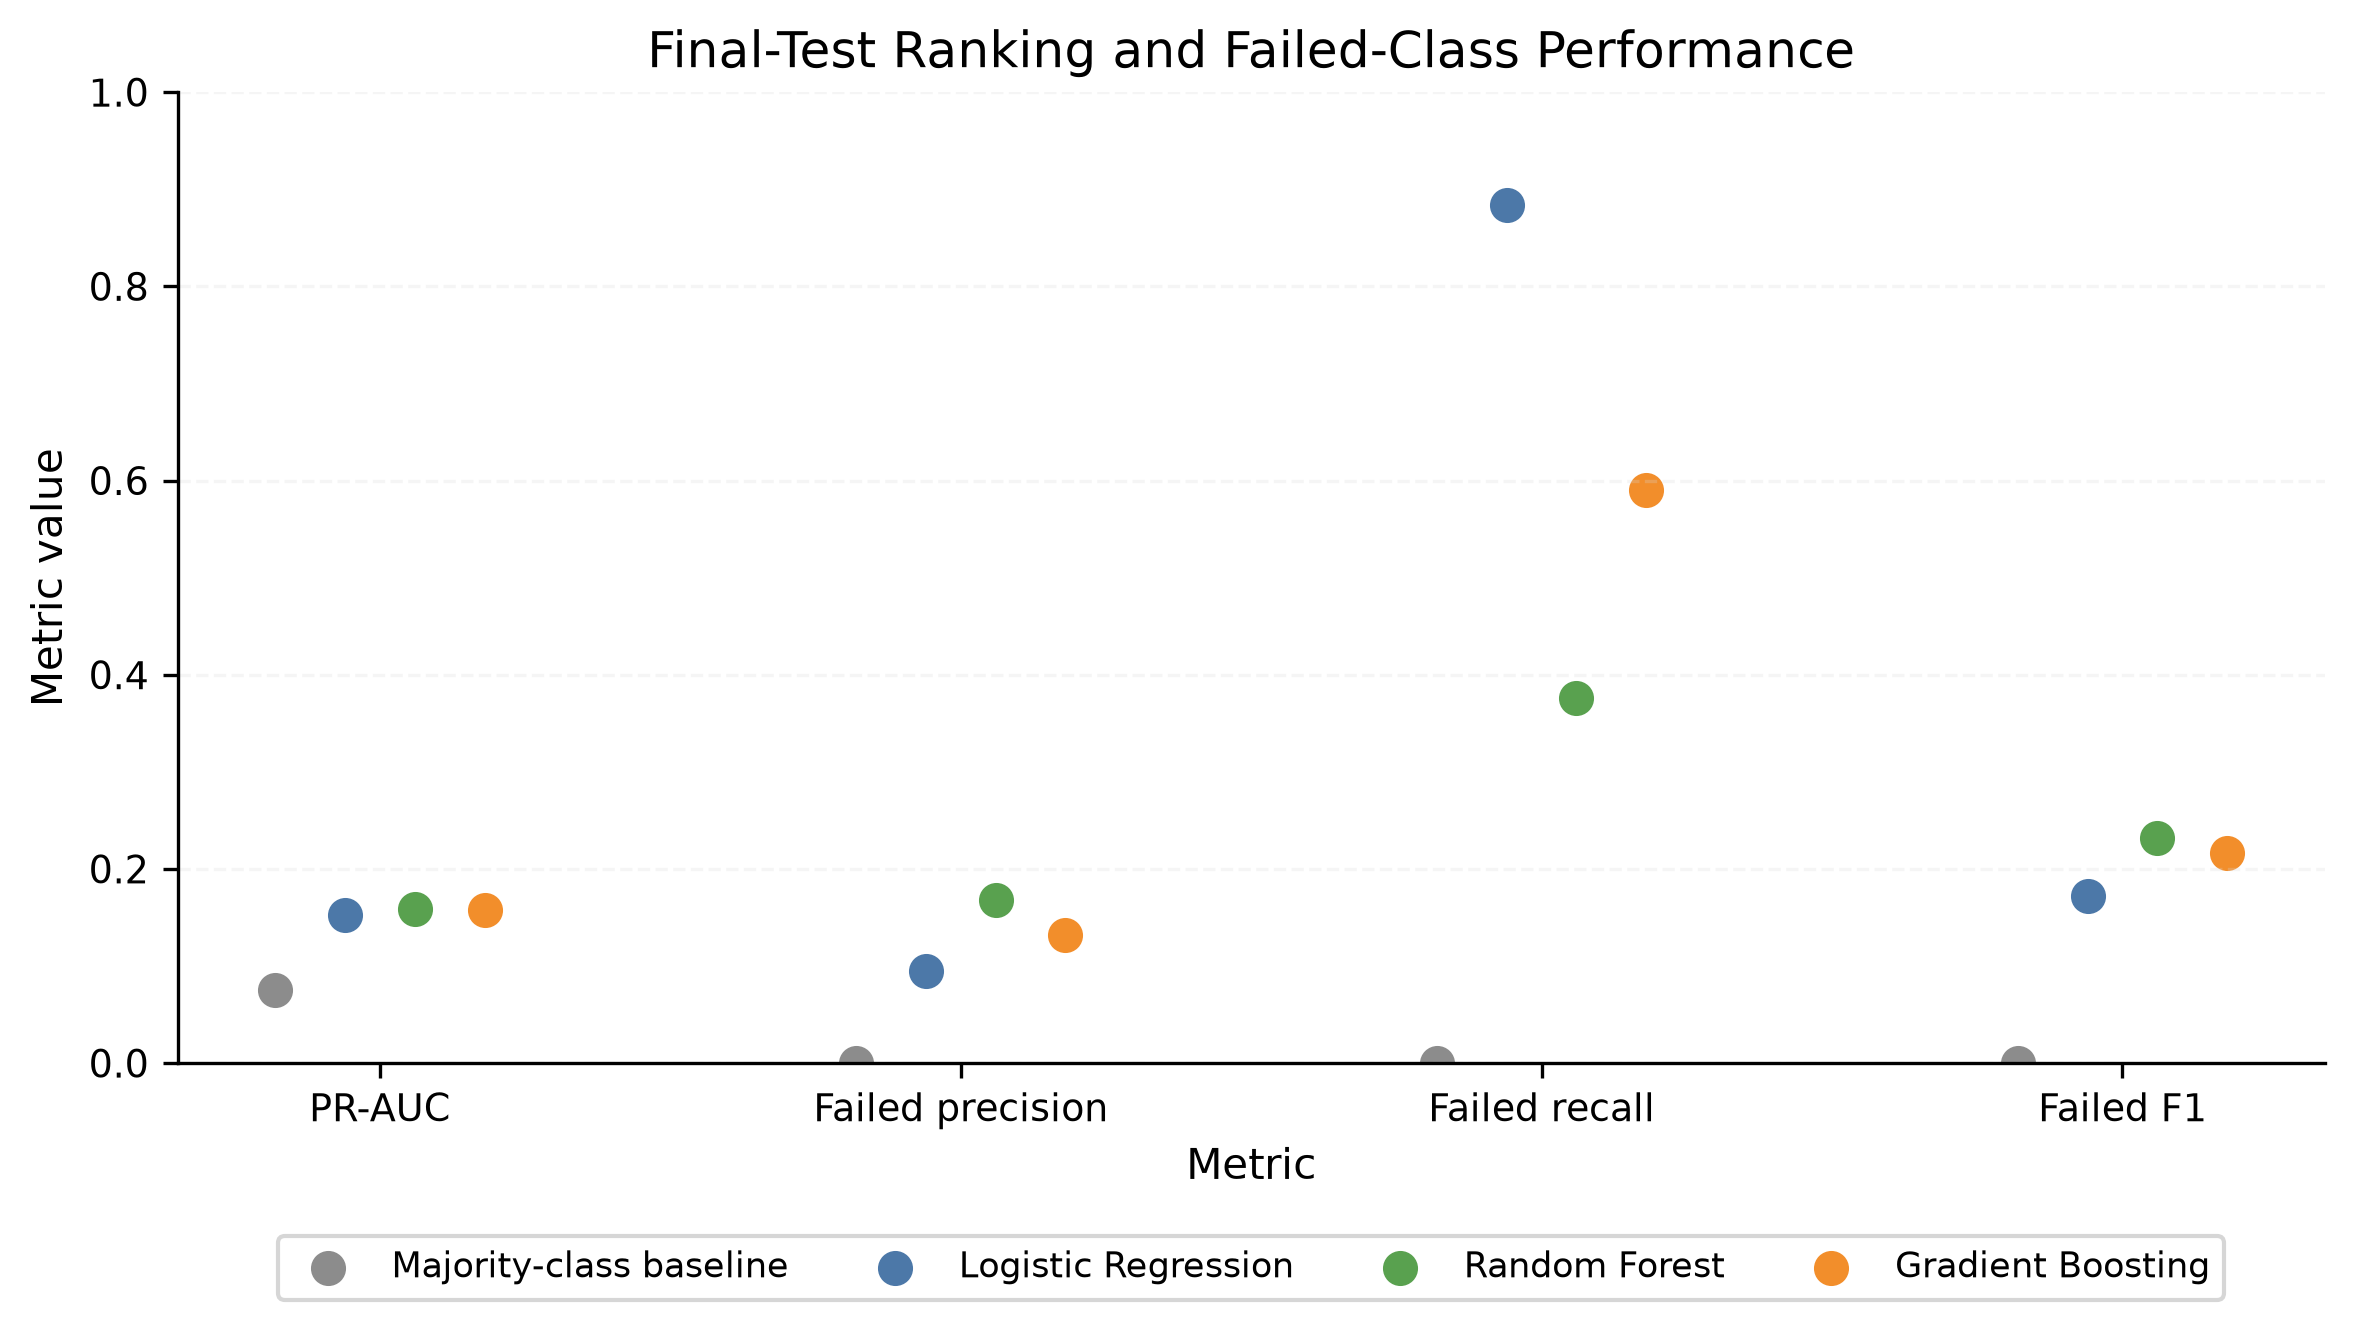
\includegraphics[width=0.82\textwidth]{model_performance_summary.png}
  \caption{Final-test performance for the failed class. PR-AUC refers to
    average precision. The values come from the fixed held-out test set.}
  \label{fig:test-performance}
\end{figure}

The majority baseline reaches 0.925 accuracy, but it detects none of the 1,177
failed observations. Its failed-class precision, recall, and F1-score are all
zero. This confirms that accuracy alone gives the wrong impression in this
imbalanced problem.

No model is strongest on every measure. Logistic Regression has the highest
failed recall at 0.884, but its failed precision is only 0.095. In plain terms,
it catches many failures by flagging many firms. Random Forest has the
numerically highest observed final-test PR-AUC among the models shown at 0.159
and the highest failed-class F1-score at 0.232. This result was observed on the
final test set and does not change the earlier model-selection decision.
Gradient Boosting has the highest balanced accuracy at 0.638 and an
intermediate recall of 0.590. The ROC-AUC values of the three models are close,
ranging from 0.688 to 0.699. Overall, the models perform differently depending
on the metric being considered.

\subsection{Classification trade-offs}

Table~\ref{tab:test-confusion} shows the final-test predictions as practical
screening results. Logistic Regression detects 1,041 failures and misses only
136. However, it also creates 9,906 false alarms. This explains why its recall
is high while its precision and overall accuracy are low. Balanced class
weighting helps explain this result. Failed observations receive more
influence during fitting, so the fitted model screens broadly at the default
decision rule. The 0.50 rule is a conventional comparison point rather than an
economically optimized threshold.

\begin{table}[H]
  \centering
  \caption{Final-test classification outcomes at the default decision rule}
  \label{tab:test-confusion}
  \small
  \begin{tabular}{lrrrr}
    \toprule
    Model & Correct alive & False alarms & Missed failures & Detected failures \\
    \midrule
    Majority baseline    & 14,517 & 0     & 1,177 & 0     \\
    Logistic Regression  & 4,611  & 9,906 & 136   & 1,041 \\
    Random Forest        & 12,327 & 2,190 & 735   & 442   \\
    Gradient Boosting    & 9,954  & 4,563 & 482   & 695   \\
    \bottomrule
  \end{tabular}
\end{table}

Random Forest is more selective. It reduces false alarms to 2,190, but detects
only 442 failures and misses 735. Gradient Boosting lies between these two
patterns, with 695 detected failures and 4,563 false alarms. In practical
terms, Logistic Regression flags the most companies, Random Forest gives fewer
alerts, and Gradient Boosting lies between them. Which pattern
is preferable depends on the relative cost of a missed failure and a false
alarm. Those costs are not estimated in this project.

The validation threshold analysis shows the same trade-off. For each
model, validation-based scenarios that reach at least 80\% recall label a much
larger share of observations as failed than the maximum-F1 scenario. Recall can
therefore be increased, but this comes with lower precision and more firms sent
for further review. These cut-offs were studied on validation data only. They
are not used to revise the final-test results above.

\subsection{Precision--recall analysis}

Figure~\ref{fig:test-pr} shows the precision--recall curves for the three key
models. The dashed horizontal line represents the failed-class share in the
test data. A curve above this line shows better ranking than a non-informative
classifier at that recall level.

\begin{figure}[H]
  \centering
  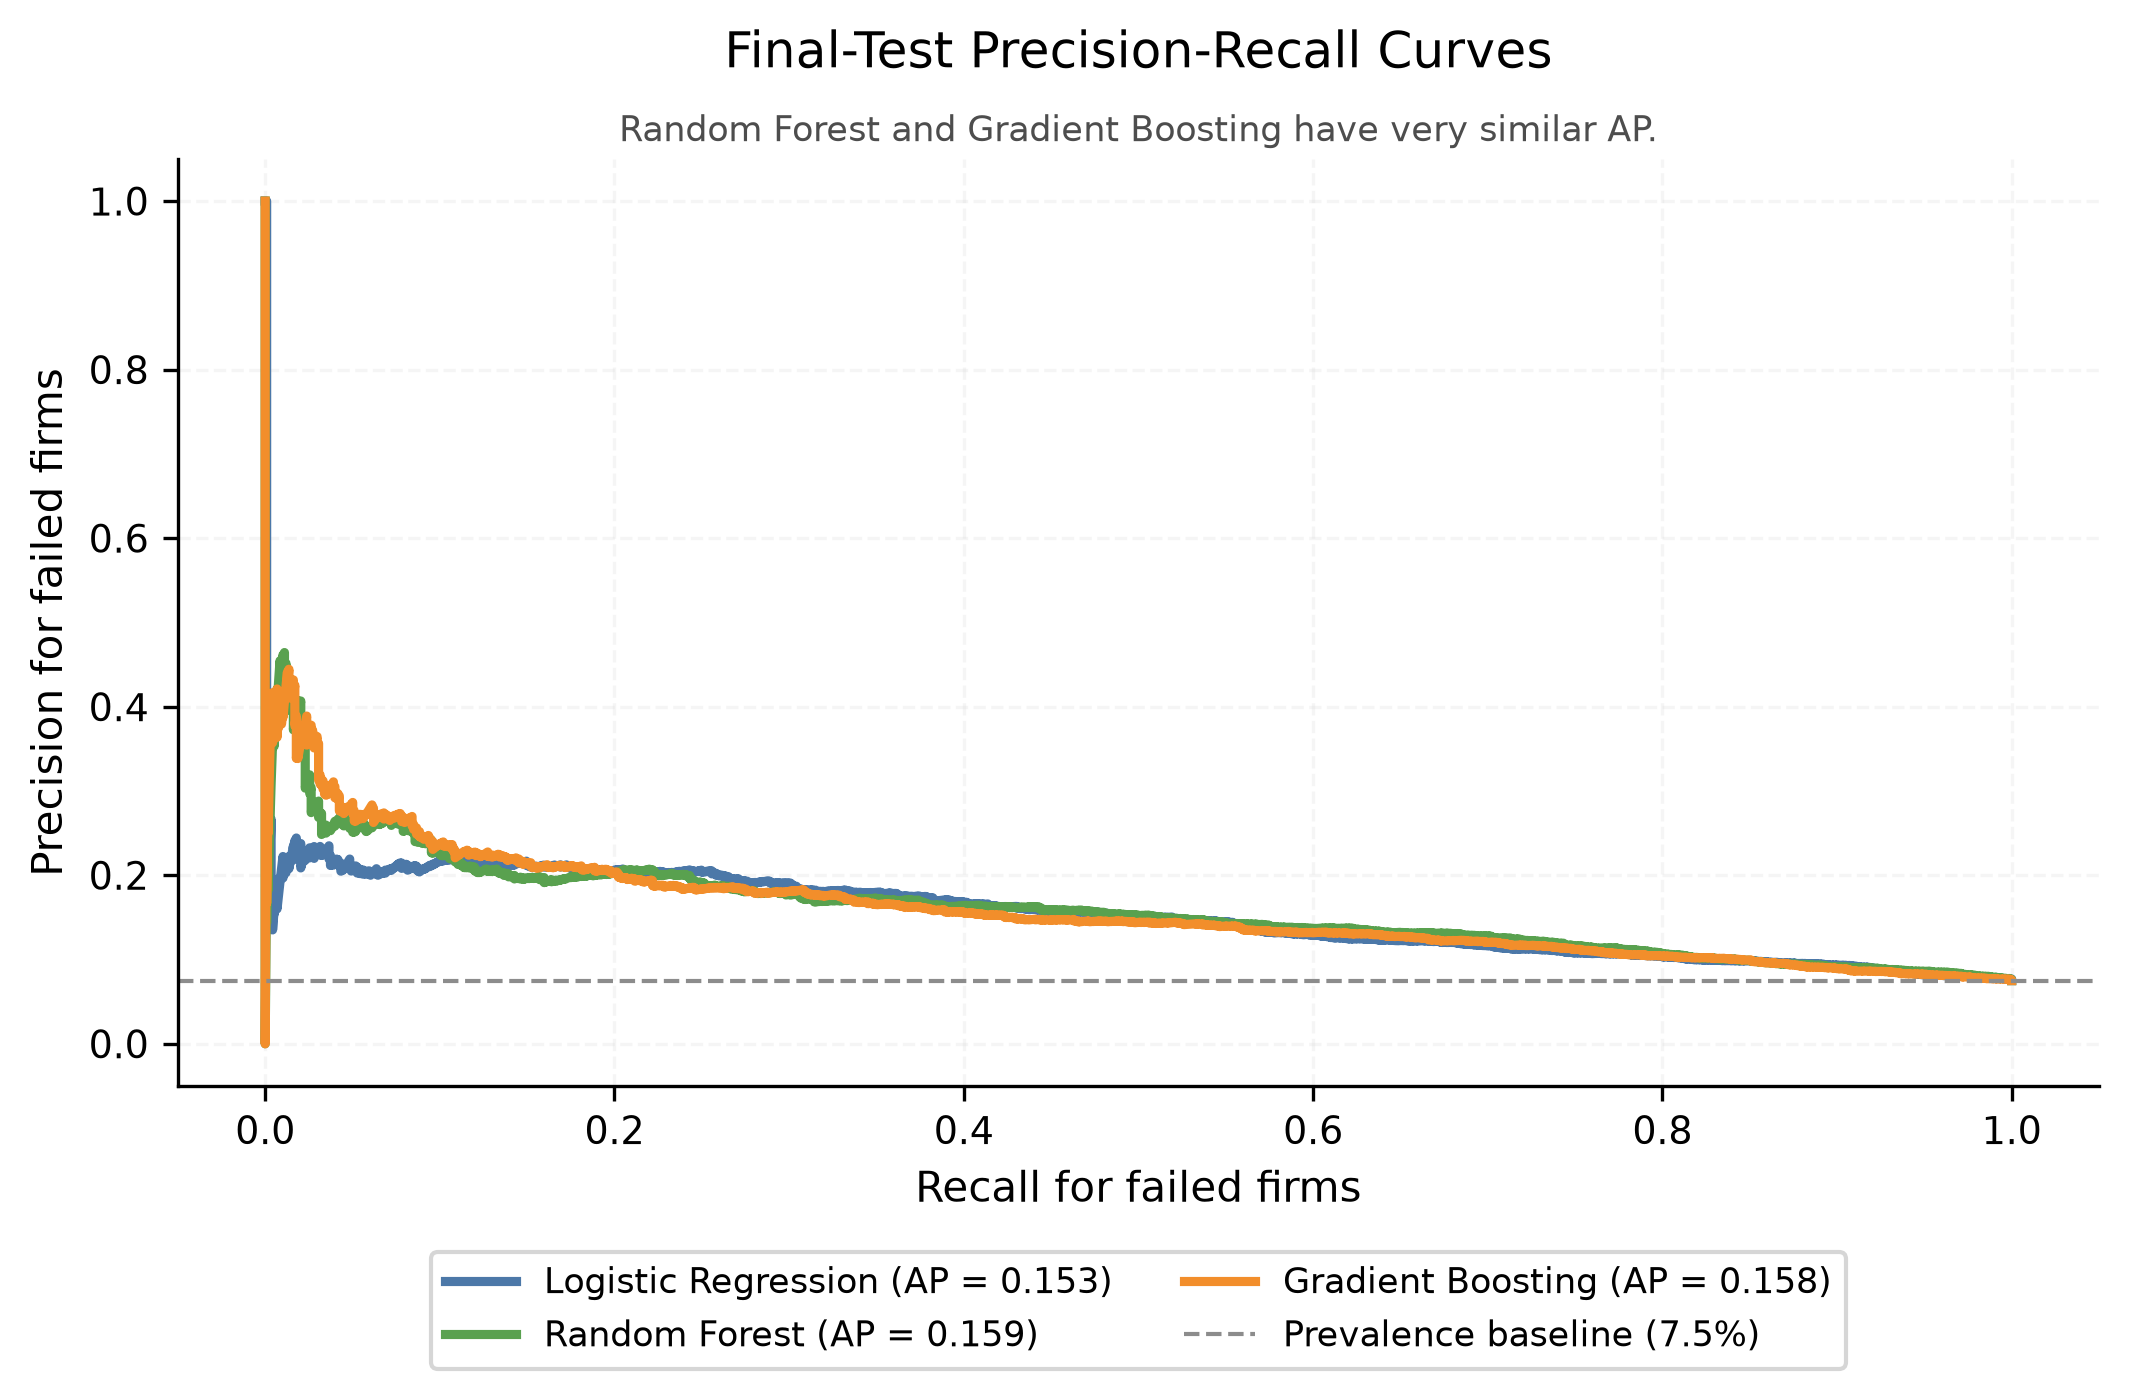
\includegraphics[width=0.74\textwidth]{precision_recall_key_models.png}
  \caption{Final-test precision--recall curves for the key models. The legend
    reports average precision, labelled PR-AUC in the project outputs.}
  \label{fig:test-pr}
\end{figure}

The curves are close. Their average precision values are 0.153, 0.159, and
0.158. Random Forest is numerically highest, but its advantage over the
validation-selected Gradient Boosting model is very small. Logistic Regression
has similar ranking performance, but its default-threshold classifications
produce a very different confusion matrix. This shows why ranking quality and
threshold-based decisions must be discussed separately. Overall, the models
contain useful predictive information, but the low precision values show that
identifying failed companies remains difficult.

\section{Model Interpretation}
\label{sec:interpretation}

\subsection{Logistic Regression coefficients}

Figure~\ref{fig:logistic-coefficients} shows the largest coefficients from the
main Logistic Regression. Because the predictors were standardized before
fitting, the coefficient sizes can be compared more directly.
Positive coefficients are associated with higher predicted failure log-odds.
Negative coefficients are associated with lower predicted failure log-odds.
These relationships are interpreted while the other predictors are kept constant.

\begin{figure}[H]
  \centering
  
\includegraphics[width=0.76\textwidth]{top_logistic_coefficients.png}
  \caption{Largest Logistic Regression coefficients. Predictors are
    standardized, and the target value one represents a failed observation.}
  \label{fig:logistic-coefficients}
\end{figure}

Current assets and market value have the largest negative coefficients, at
$-1.912$ and $-1.812$. EBIT, retained earnings, and EBITDA also have negative
coefficients among the variables shown. In this fitted model, higher values of
these variables are associated with lower predicted failure risk. This is
also similar to the descriptive results, where failed observations have lower
median current assets, market value, net income, and retained earnings.

Total current liabilities have the largest positive coefficient at 0.928.
Depreciation and amortization, gross profit, inventory, and total assets also
have positive coefficients among the largest values. These coefficient signs
should be interpreted carefully. The model includes several related accounting totals at the same
time. A coefficient therefore describes a conditional relationship after the
other variables are held fixed. For example, the positive gross-profit
coefficient should not be read as evidence that higher gross profit causes
bankruptcy. The positive sign may result from the way gross profit is related
to company size, revenue, costs, and balance-sheet variables in the fitted model.

The coefficients help explain how the model forms its scores, but they are not
causal estimates. The analysis also does not report statistical inference for
individual coefficients. They are used here only to explain the model's
predictions.

\subsection{Tree-based feature importance}

Figure~\ref{fig:tree-importance} reports the leading impurity-based feature
importance values for Random Forest and Gradient Boosting. A larger value means
that the variable contributed more to reducing impurity when the model created
splits. Unlike a logistic coefficient, this measure does not show whether higher
values increase or decrease predicted risk.

\begin{figure}[H]
  \centering
  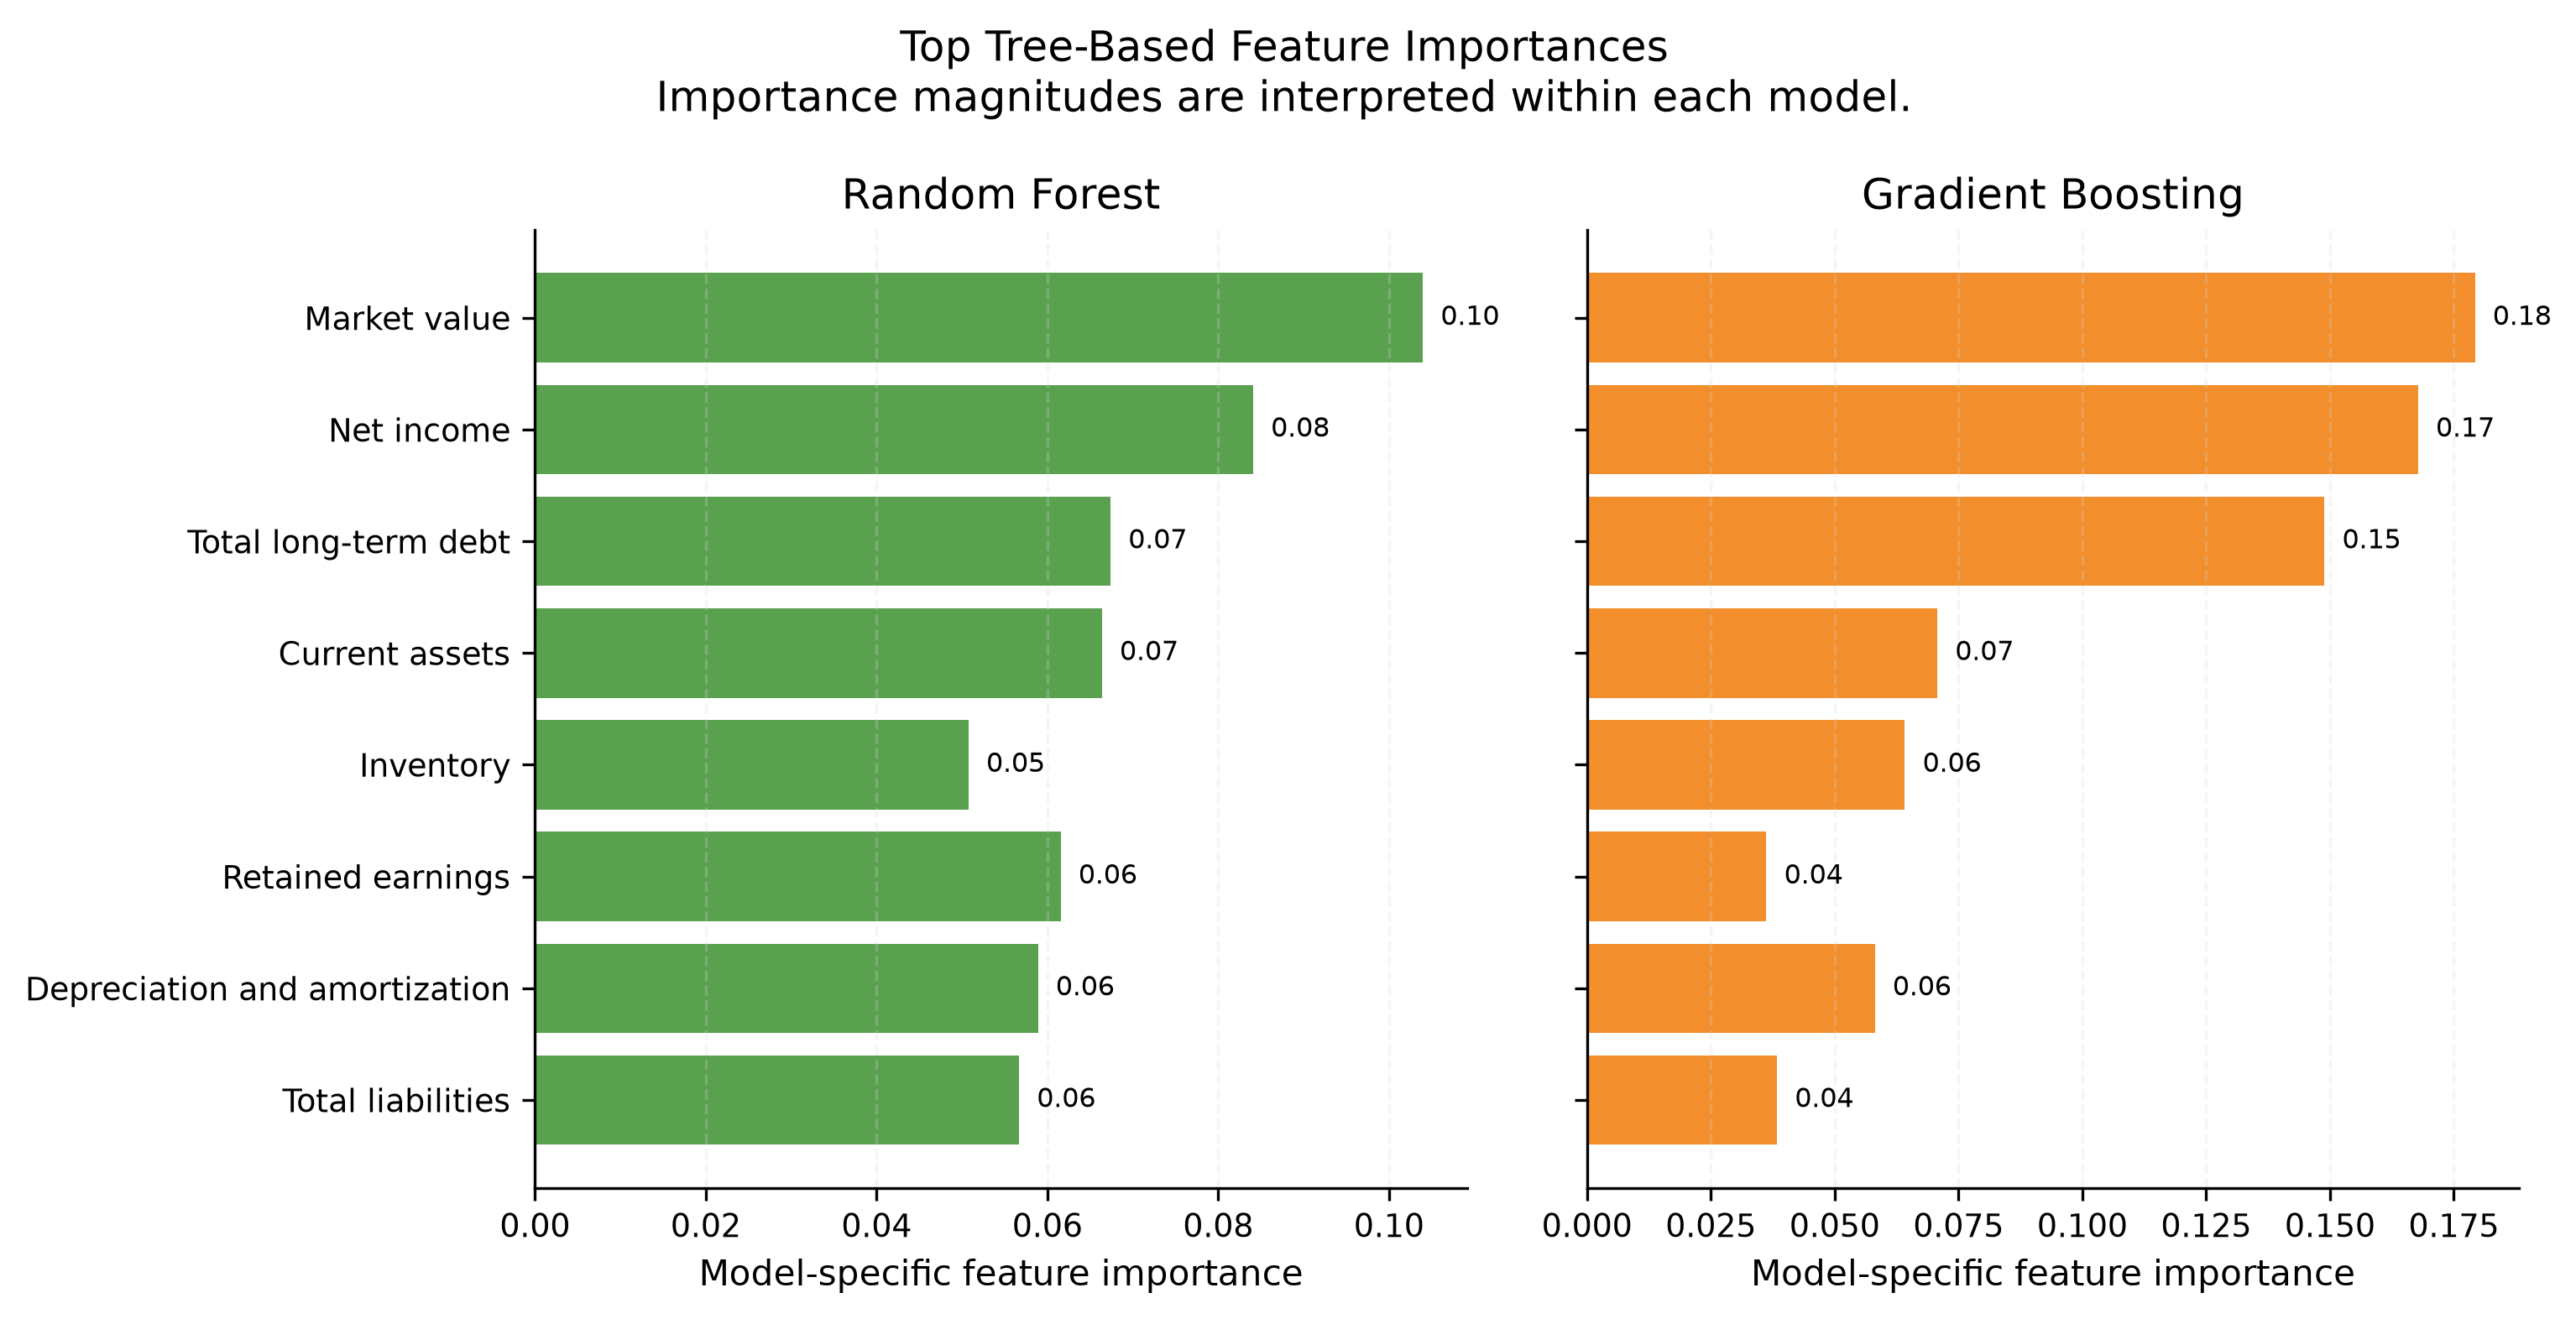
\includegraphics[width=0.80\textwidth]{top_tree_feature_importance.png}
  \caption{Leading feature importance values within the Random Forest and
    Gradient Boosting models. Magnitudes should be compared mainly within each
    model rather than directly across models.}
  \label{fig:tree-importance}
\end{figure}

Market value, net income, and total long-term debt are the three most important
features in both ensembles. Current assets also appear near the top, followed
by variables such as inventory, depreciation and amortization, and total
liabilities. Retained earnings is also prominent in the Random Forest. This
overlap suggests that market valuation, profitability, liquidity, and debt
information all contribute to the models' predictions. It does not establish
that these variables cause failure.

The two models also distribute importance differently across the variables. Random Forest spreads
importance more evenly across the predictors, while Gradient Boosting assigns
a larger share to its first few variables. The absolute values should not be
compared as if they were on one common scale. Each ensemble constructs and
combines trees differently. Impurity-based importance can also favour variables
that provide many useful split points. When predictors are correlated, importance
can be divided across related variables. The figure should therefore be used to
describe the fitted models, not to rank the economic causes of bankruptcy.

Taken together, the two interpretation methods offer different information.
Logistic Regression provides signed and relatively direct relationships on the
log-odds scale. The ensembles allow nonlinear patterns and interactions, but
their importance values are less direct. This shows the main trade-off between
model flexibility and interpretability in the project. More flexible models can represent richer patterns,
while the logistic model is easier to explain in financial terms.

\section{PCA Results}
\label{sec:pca-results}

The PCA analysis examines whether the 18 standardized financial variables can
be reduced without losing much predictive information. The first few components
explain a large share of predictor variation. Two components retain 83.8\% of
total variance, five retain 93.9\%, and ten retain 99.2\%.

A high explained variance does not automatically mean strong classification
performance.
Table~\ref{tab:pca-results} reports the internal validation results for PCA
followed by Logistic Regression. With only two components, ROC-AUC is 0.498 and
PR-AUC is 0.063, even though those components retain most of the predictor
variance. Performance improves when more components are included. The
ten-component version has the highest failed-class F1-score, at 0.152. The
twelve-component version has the highest PR-AUC, at 0.151. These differences
are small.

\begin{table}[H]
  \centering
  \caption{Internal validation results for PCA with Logistic Regression}
  \label{tab:pca-results}
  \small
  \begin{tabular}{rrrrr}
    \toprule
    Components & Explained variance & ROC-AUC & PR-AUC & Failed F1 \\
    \midrule
    2  & 0.838 & 0.498 & 0.063 & 0.130 \\
    3  & 0.892 & 0.642 & 0.116 & 0.146 \\
    5  & 0.939 & 0.651 & 0.124 & 0.148 \\
    8  & 0.980 & 0.669 & 0.140 & 0.150 \\
    10 & 0.992 & 0.671 & 0.147 & 0.152 \\
    12 & 0.998 & 0.674 & 0.151 & 0.150 \\
    15 & 1.000 & 0.671 & 0.147 & 0.149 \\
    18 & 1.000 & 0.671 & 0.147 & 0.149 \\
    \bottomrule
  \end{tabular}
\end{table}

For comparison, Logistic Regression on the original standardized predictors
has a validation PR-AUC of 0.148 and a failed-class F1-score of 0.149. The PCA
models with ten or twelve components therefore perform similarly, but they are
not clearly better. PCA can reduce the input dimension. However, reducing the
data to only two or three components removes information that appears useful
for distinguishing failed and alive observations.

PCA also makes the results harder to interpret in financial terms. Each component is a weighted
combination of many accounting variables, so it cannot be discussed as
directly as current assets, market value, income, or debt. In this project, the
small improvement on the validation sample is not enough to justify the weaker
interpretation. The PCA analysis is still useful because it shows that
explaining predictor variation is not the same as predicting bankruptcy well.
All PCA comparisons are validation results only. They are not used to make any
additional conclusions about final-test performance.

\section{Critical Reflection and Limitations}
\label{sec:limitations}

The project includes several choices that strengthen the analysis. Splitting by
company prevents the same firm from appearing in both training and test data.
Keeping the test set separate from model selection and threshold analysis also
makes the final comparison more reliable. Finally, the majority baseline and
failed-class metrics expose weaknesses that would be hidden by accuracy. These
choices make the comparison cleaner, but they do not remove the following
limitations.

\subsection{Data and target limitations}

The data contain repeated company-year observations. Observations from one firm
are likely to be related over time. The company-level split handles direct firm
overlap, but the design is not a chronological forecasting exercise. The
training and test samples cover overlapping calendar years. The results
therefore show how well the models work for unseen companies in a similar
historical period, not how well they would perform in a later period. The changing annual failure
rate also suggests that time and sample composition matter.

The failed/alive label is suitable for classification, but the future period
being predicted is not clearly defined. A real early-warning application
would need a statement such as ``failure within the next twelve months'' and
would need to confirm that every accounting variable was available before that
forecast date. Without this timing detail, the results should be read as
classification of company-year observations, not as a complete real-time
forecasting exercise.

The predictors are financial statement levels. They contain information about
firm condition, but they may also partly reflect company size and accounting
scale. This matters because large firms naturally have larger assets,
liabilities, sales, and expenses. The project does not add financial ratios,
changes over time, industry indicators, macroeconomic conditions, governance
information, or market returns. Dataset coverage and reporting choices may also
make the sample different from other countries, private firms, or later periods.
For this reason, the results may not apply in the same way to other datasets or
settings.

\subsection{Validation and modelling limitations}

The reported results come from one grouped train--test split and one internal
validation split. They do not show how much performance would vary under other
valid splits. There are no confidence intervals, repeated grouped validation,
or statistical tests of the small differences between models. In particular,
the very close PR-AUC values do not prove that one ensemble model is generally
better than the other.

The hyperparameter searches are limited so that the project remains manageable,
but better settings may still exist. The saved
final models are also fitted on the inner model-training portion and are not
refitted after validation. This means that some available training observations
are not used in the final model. It is also less data-efficient. A
later version could lock all choices, refit on the complete non-test sample, and
then evaluate once on a still-unused test set.

The models evaluate discrimination and classification, not probability
calibration. Their outputs should therefore not automatically be interpreted
as literal bankruptcy probabilities. Interpretation also has limits. Logistic
coefficients can change when correlated predictors are included together.
Impurity-based tree importance has its own biases. Both are descriptions of
fitted predictive models, not causal evidence.

\subsection{Decision and practical limitations}

The threshold analysis makes the precision--recall trade-off visible, but the
project does not estimate the monetary cost of a missed failure or a false
alarm. It also does not specify how many flagged firms an analyst could review.
Without clear financial costs or a limit on how many cases can be reviewed, it
is not possible to identify one best model or threshold. The low failed-class precision is especially
important: even the more selective models produce many false alerts.

A real financial application would require further checks, including
probability calibration, chronological backtesting, stability across industries
and economic conditions, stress testing, fairness and governance review, and a
plan for monitoring model drift. Human review would also be necessary before any
credit, investment, or regulatory action. The current project is a reproducible
educational study and screening exercise. It is not production-ready.

\subsection{Priorities for future work}

The most important improvement would be to define a clear forward failure
horizon and use rolling or chronological evaluation. Repeated company-grouped
validation and uncertainty intervals would show whether model differences are
stable. Financial ratios and trends could reduce the influence of firm size,
while industry and macroeconomic variables could add context. After model
selection, probability calibration should be tested, and the threshold should be
chosen using explicit financial costs and review capacity. These improvements
would be more useful than simply adding another complex model.

\section{Conclusion}
\label{sec:conclusion}

This paper examined whether financial statement variables can help identify
failed observations for companies that were not used during model fitting. It
compared interpretable and tree-based classifiers for company-year
bankruptcy-risk classification. The results show that the financial variables
contain useful information for distinguishing failed and alive observations
under the company-level split. However, bankruptcy classification remains
difficult, and the best model depends on the goal of the analysis.

The majority-class baseline achieved 92.5\% accuracy while detecting no failed
observations. This shows why accuracy alone is insufficient. Among the key
models, Logistic Regression had the highest failed recall, but it also produced
many false positives. Random Forest produced the numerically highest observed
final-test PR-AUC and failed-class F1-score. Gradient Boosting was the
validation-selected model and had the highest balanced accuracy. This
is important because the final test set is used only for evaluation and not to
select the model afterward.

The additional analyses show the same general pattern. Validation threshold
analysis showed that higher recall requires lower precision and more review
effort. PCA reduced the number of inputs but did not clearly improve validation
performance. Logistic Regression coefficients and tree-based feature importance
helped explain the fitted models, especially for valuation, profitability,
liquidity, and debt variables, but these relationships are not causal. Overall,
the models are useful for screening companies in this course project, but they
should not be used for automatic financial decisions or as a production system.
A future study should define a clear prediction period, use chronological
evaluation, test calibration and uncertainty, and choose thresholds based on
financial costs and review capacity.

% -----------------------------------------------------------------------------
% References
% -----------------------------------------------------------------------------
\bibliographystyle{apalike}
\IfFileExists{references.bib}
  {\bibliography{references}}
  {\section*{References}}

\end{document}
